\documentclass[11pt]{article}
\usepackage{mgates-letter}
\definecolor{dark_blue} {rgb}{0., 0., 0.65}
\usepackage{makecell}
\usepackage{listings}
\usepackage{textcomp}
\usepackage{boxedminipage}
\usepackage{rotating}
\usepackage{csquotes}
\usepackage[font={small}]{caption}
\usepackage{acronym}
%\usepackage{natbib}
\usepackage[colorlinks, filecolor=dark_blue, urlcolor=dark_blue, linkcolor=black, citecolor=black]{hyperref}
\usepackage[
	backend=biber,
	style=numeric,
	url=false
]{biblatex}
\usepackage{cleveref}
\defbibcheck{mine}{\iffieldundef{annotation}{\skipentry}{}}
\defbibcheck{other}{\iffieldundef{annotation}{}{\skipentry}}

\addbibresource{biblio.bib}
\lstdefinelanguage{scala}{
  keywords={abstract,case,catch,class,def,%
    do,else,extends,false,final,finally,%
    for,if,implicit,import,match,mixin,%s
    new,null,object,override,package,%
    private,protected,requires,return,sealed,%
    super,this,throw,trait,true,try,lazy,%
    type,val,var,while,with,yield,forSome},
  otherkeywords={=>,<-,<\%,<:,>:,\#},
  sensitive=true,
  morecomment=[l]{//},
  morecomment=[n]{/*}{*/},
  morestring=[b]",
  morestring=[b]',
  morestring=[b]""",
  basicstyle=\lst@ifdisplaystyle\small\fi\ttfamily,
  emphstyle=\bfseries
}
\definecolor{ddarkgreen}{rgb}{0,0.5,0}
\lstdefinelanguage{scafi}{frame=single,basewidth=0.5em,language={scala},
keywordstyle=\color{blue}\textbf, commentstyle=\color{ddarkgreen},
keywordstyle=[2]\color{red}\textbf, keywords=[2]{rep,nbr,foldhood,foldhoodPlus,aggregate,branch,spawn,mux,mid},
keywordstyle=[3]\color{gray}, keywords=[3]{Me,AroundMe,Everywhere,Forever}, %,@@,@@@
keywordstyle=[4]\color{red}\textbf, keywords=[4]{in,out,rd},
keywordstyle=[5]\color{violet}, keywords=[5]{evolve,when,andNext,workflow,G,C,broadcast,gossip},
keywordstyle=[6]\color{orange}, keywords=[6]{Available,Serving,Done,Waiting,Removing,None,Set}}
\lstset{language=scafi}

\begin{document}
\sloppy
\begin{center}
	{{
		\Large{
			\textsc{PhD Programme in Computer Science and Engineering \\ 
			\vspace{4mm}
			Cycle XXXVI}
			}
	}} 
	\rule[0.1cm]{\textwidth}{0.1mm}
	\rule[0.4cm]{\textwidth}{0.6mm}
\end{center}

\begin{center}
	{\LARGE{A Language-based Software Engineering Approach for Cyber-Physical Swarms}} \\
	\vspace{4mm}
	{\large{PhD Thesis proposal}} 
	\vspace{4mm}
\end{center}
\vspace{8mm}
\par
\noindent
\begin{minipage}[t]{0.47\textwidth}

{\large{Commission: \\\bf
Prof. Mirko Viroli \\
Prof. Andrea Omicini \\
Prof. Matteo Ferrara} 
}
\end{minipage}
\hfill
\begin{minipage}[t]{0.47\textwidth}
	\raggedleft
	{
		\large{PhD Student: \\\bf Gianluca Aguzzi}
	}
\end{minipage}
\vspace{10mm}

{
	\raggedright
	\rule[0.1cm]{\textwidth}{0.6mm}
	\rule[0.5cm]{\textwidth}{0.1mm}
}

\newcommand{\scafiweb}{{ScaFi-Web}}
\acrodef{ac}[AC]{Aggregate Computing}
\acrodef{cpsw}[CPSw]{Cyber-Physcal Swarm}
\acrodef{marl}[MARL]{Multi-Agent Reinforcement Learning}
\acrodef{rl}[RL]{Reinforcement Learning}
\acrodef{ml}[ML]{Machine Learning}
\newcommand{\agcfull}{{aggregate computing}}
\newcommand{\agc}{{AC}}
\newcommand{\marl}{{MARL}}
\newcommand{\rl}{{RL}}
\newcommand{\scafi}{{ScaFi}}
\newcommand{\cpsw}{{CPSw}}
\newcommand{\rev}[1]{{
	%\color{red}
	#1
	}}
\abstract{
	This thesis aims to define a path towards the engineering of \textit{\acp{cpsw}} - where artificial swarms are seen in a modern key, including swarm robotics, large-scale IoT scenarios, and crowd engineering (tracking and control). 
	%
	\acp{cpsw} are backed by emerging trends of autonomic, pervasive, ubiquitous computing that foster a vision of distributed systems composed of a considerable number of simple entities that collectively perform collective tasks.
	%
	These systems are similar to social animal groups, where plentiful individuals (like ants, sheep, \dots) realise shared population-wide goals.
	%
	Furthermore, these behaviours are typically achieved through self-organisation, making the system robust to failures and highly scalable.
	%
	Inspired by nature, I define the notion of \acl{cpsw} -- the extension of natural `swarm' in Computer Science.
	%
	Engineering these systems with traditional approaches is inadequate, 
	due to the distributed control, high-rate failure, openness, and local-to-global behaviour mapping.
	%
	Therefore, my thesis is focused on finding a systematic and reproducible way to design \acp{cpsw}.
	In particular, I plan to follow a language-based approach, where the models and tools are built around a target programming language. 
	%
	In this case, I decided to leverage \ac{ac} -- a novel top-down global-to-local programming model.
	%
	As a final result of my PhD, I intend to analyse the application of \ac{ac} in \acp{cpsw}. 
	%
	This will touch on several aspects like distributed intelligence, flexible and opportunistic middleware, building blocks and ad hoc API definition.
}
\acresetall
\newpage
%\tableofcontents
\section{Introduction}
The recent evolution of IT technologies fosters a vision in which computation is \textit{everywhere}. 
%
Several modern paradigms advance that vision, like ubiquitous~\cite{DBLP:journals/sigmobile/Weiser99}, pervasive~\cite{DBLP:journals/computer/SahaM03}, collective~\cite{DBLP:journals/computer/Abowd16}, and automatic computing~\cite{DBLP:journals/computer/KephartC03}.
%
These paradigms take into account systems (typically \emph{cyber physical}) where a large number (hundreds - thousands - millions) of simple interacting devices collectively perform complicated tasks in a decentralised manner, acting and sensing through a shared environment. 
%
Thus, they can be conceived as \textit{complex} systems like the ones observed in nature.
%--  by means that we cannot understand the behaviour of the whole looking only at the parts.
%
Speaking about \textit{natural} complex systems, social animals, like a swarm of insects, exhibit fault-tolerant, effective, and efficient collective behaviours leveraging self-organisation.

Consequently, I want to promote cyber-physical systems with the properties observed in swarms, thus I came to define \acfi{cpsw}: a collection of (simple) computational entities linked with the physical world via perception and actuation that reach collective goals through self-organising behaviours.
%
Swarm robotics, ``swarms” of people (crowds) or, in general, ``swarms” of IoT devices are clearly defined instances of \acp{cpsw}.
%
Traditional design methodologies (device-level) are inadequate for \acp{cpsw} engineering, due to local-to-global mapping problems, distributed control, complex IT infrastructures, and scalability concerns.
%
To overcome these issues, the goal of my research PhD thesis is to find a systematic methodology (models, techniques and algorithms) to synthesise and deploy self-organising behaviours with predictable outcomes for \acp{cpsw}.

This is not the first effort that wants to tackle these kinds of problems. 
%
Traditionally, designers have been guided by natural phenomena observation that was then transposed into computer systems -- a so-called bottom-up approach. 
%
However, this methodology led to specific solutions that hardly scale up with application complexity.
%
Novel techniques -- and the one that I follow in this work -- consist of top-down global-to-local approaches where designers define the system outcome directly at the collective level.
%
Among the many (like Buzz~\cite{DBLP:journals/software/PinciroliB16}, TOTA~\cite{DBLP:conf/icdcsw/MameiZL03}) in this thesis, I will take into consideration \acfi{ac}~\cite{DBLP:journals/computer/BealPV15} since it enables the definition of self-organising collective behaviours that can be functionally composed. 
%
In this way, the \textit{aggregate} programs (i.e. programs written using \ac{ac}) can be reused in different domains and can scale with application complexity. 

Even if \ac{ac} is already applied in different scenarios like crowds of people~\cite{DBLP:journals/computer/BealPV15}, smart cities~\cite{DBLP:journals/isci/CasadeiFPRSV19}, and large-scale IoT~\cite{DBLP:journals/fgcs/CasadeiFPRSV19}, it currently lacks a software architecture (middleware), systematic program definition, abstraction layers (API) and foundational aspects.
%
Consequently, my thesis aims to investigate and critically analyse \ac{ac} techniques in the field of \acp{cpsw}.
%
This investigation will cover multiple directions like distributed intelligence, flexible middlewares, and ad-hoc building blocks, possibly leading to contributions both at a foundational (i.e., building blocks, \ac{ac} language, API) and architectural level (middleware, message passing architecture, ...).
%
In this process, \ac{ml} -- and in particular \ac{rl} -- techniques will be used in support of \ac{ac}~\cite{research} to improve adaptivity, efficiency, and efficacy.

The proposal is then structured as follows. In \Cref{background} I discuss the current state-of-the-art methodologies and related works in the field \acp{cpsw} behaviour definition.
%
In \Cref{contribution} I devise my thesis contribution in the path of engineering predictable outcome in \acp{cpsw}. 
%
In this section, I also show the preliminary works done in this first PhD year.
%
Finally, in \Cref{future} I describe what are the activities that I plan to do in the rest of my PhD project.

\section{Background} \label{background}
The goal of this section is to clarify what I mean by \textit{Cyber-Physical Swarms}, what systems are similar to our definition, and which research areas have to deal with similar problems.
\subsection{Cyber-Physical Swarms}
This term is used to describe many computational nodes that collaborate to solve collective problems, similarly to what we observe in natural ``swarm'' systems.
%
These systems have a large population of networked nodes (hundreds -- thousands), and they are typically \textit{open} (i.e. we cannot know the total node number apriori). 
%
Consequently, the collective behaviour should be \textit{scale-independent} (i.e. the same program must work in small networks as well as in very large networks).
%
Besides, nodes are associated with a \textit{physical} asset through sensors and could change the environment using actuators. 
%
Namely, they have an \emph{embodiment} in the world -- so the name of cyber-physical. 
%
The nodes could be heterogeneous, but with a \emph{homogenous} local behaviour (i.e., each node should execute the same local logic). 
%
Furthermore, nodes act collaboratively, and they are not selfish -- they always operate for the global collective good.
%
I suppose that the overall system could not use a central entity -- so I need to deal with a distributed control. 
%
Even if modern architectures could be used (e.g cloud/edge infrastructures), in general, the system needs to react to local problems quickly. 
%
Hence, moving this decision far from the physical assets could be dangerous (since they are a kind of \emph{critical systems}).
%
As a concluding note, I want to consider their behaviour at the \textit{macro-level}, not at the \text{micro-level}. 
%
Hence, I intend to describe the collective not by emergence, but by defining a global wanted structure.

\acp{cpsw} are kind of Complex Adaptive systems~\cite{holland1992complex}, but our vision enforces properties that are not necessarily present in standard complex systems' definition, like the large agents' number and the collaborative agents' nature.
%%
Collective Adaptive Systems~\cite{DBLP:journals/corr/abs-1108-5643} are near to our \acp{cpsw} description but in our definition agents pursue \emph{collective} (not individual) goals, and they have a homogenous behaviour.

\subsection{Swarm Intellingence}

Swarm Intelligence has a similar starting point to our approach since it tries to apply the tactics observed in social animals in swarm robotics. 
%
The behaviours are derived in a bottom-up fashion, hence designers have tried to achieve collective behaviours through emergence observing individual animal behaviours.
%
For instance, artificial stigmergy~\cite{DBLP:journals/fgcs/DorigoBT00} derives from those studies.
%
However, nowadays, Swarm Intelligence is more focused on algorithms.
% 
Indeed, the collective behaviours observed in nature are leveraged to perform \textit{optimisation} strategies or to directly solve problems by searching in the solution space.
%%
There are several examples of Swarm Intelligence optimisation algorithms, such as Ant Colony Optimisation (ACO)~\cite{DBLP:journals/tsmc/DorigoMC96}, Particle Swarm Optimisation (PSO)~\cite{DBLP:conf/icnn/KennedyE95} and Flock of Starling Optimisation (FSO)~\cite{DBLP:series/sci/FulgineiS11}.

Even if they are important approaches, I am not directly interested in using them. 
%
Indeed, I draw \textit{inspiration} from swarms but only to achieve similar behaviour in the artificial swarm leveraging self-organisation. 
%
I do not want to \textit{mimic} nature but I aim to exploit the same mechanisms to build robust collective systems.

\subsection{Swarm Robotics}

Historically, Swarm Robotics derives from the first Swarm Intelligence approaches. 
%
Then, it has emerged as the \textit{engineering} part of that branch. 
%
Indeed, the general goal of \emph{swarm engineering} is \emph{to define systematic and well-founded procedures for modelling, designing, realising, verifying, validating, operating, and maintaining a swarm robotics system}~\cite{DBLP:journals/swarm/BrambillaFBD13}.

In Swarm Robotics, the focus is mainly on \textit{robots} that are \emph{autonomous}, \emph{situated}, and with \emph{no central control}. 
%
I aim to expand this vision also to other ``swarm-like'' systems, such as a crowd of people, large-scale IoT and smart cities where I do not have robots. 
%
In particular, the novel branch of \textit{automatic design}~\cite{DBLP:journals/firai/FrancescaB16} is very appealing to be used in \acp{cpsw}. 
%
In autonomic design approaches, the controller is derived through \textit{genetic algorithms} or \textit{Multi-agent Reinforcement Learning} following a \textit{global} utility function. 
\subsection{Multi-Agent Systems}
A \ac{cpsw} could be seen as a multi-agent system -- in particular a \emph{many}-agent system -- where a group of autonomous entities are programmed to achieve collective behaviours through \emph{repeated} sensing, computation, communication, and actuation.

Due to the high stochasticity of the environment, it is almost impossible to know and program the optimal behaviour for all agents in advance.
%
This uncertainty results in creating intelligent agents so that they can \emph{learn} the optimal behaviour and adapt to environmental changes.
\subsubsection{Learning}
In recent decades, there has been an emerging trend in the use of \ac{rl} 
in multi-agent settings -- called \ac{marl} -- as a powerful, robust and adaptive learning paradigm.
%
Progress has been considerable, and a broad number of algorithms are now available.

\ac{marl} is a conjunction of Game Theory and \ac{rl}, 
 and there are several (even orthogonal) viewpoints on which researchers have been focused on.
%
Firsts attempt from \ac{rl} viewpoint go towards a so-called \textit{independent learning}~\cite{DBLP:journals/tsmc/BusoniuBS08} approach, where each agent learns locally against the whole environment~\cite{DBLP:conf/icml/Tan93}.
%
The benefit of these approaches is that they can scale up with the number of agents, but, unfortunately, the learning process is extremely non-stationary and unstable.
%
Other efforts have focused on achieving game-theoretic properties in multi-agent settings, such as Nash equilibrium of Pareto optimality.
%
The problem is that these solutions consider typically only a few agents and hardly scale with the application complexity.
%
Emerging trends in \ac{marl} literature (both RL-based and game theoretic based) tend to leverage a so-called centralised training and decentralised execution (CTDE)~\cite{DBLP:journals/tcyb/NguyenNN20} approach, by which 
agents exploit the system-wide knowledge at training time but then at runtime they act independently~\cite{DBLP:journals/aamas/Hernandez-LealK19}. 
%
In this setting, Deep Learning is typically employed, reaching and exceeding the state-of-the-art traditional \ac{marl} algorithms.
 
The main problem with most of the solutions available in the literature is that they consider a small number of agents (or at least the algorithms are tested using a few computational nodes) --- even if some novel trends exist, like Mean Field Reinforcement Learning~\cite{DBLP:journals/corr/abs-2108-02731}.
%
Furthermore, in \acp{cpsw} I am mainly interested in learning algorithms that tackle homogenous and cooperative behaviour, i.e., the policy founded could be shared with the entire collective. 
%
This will ease the training phase with a huge agents population, reducing the non-stationary and state-action space.
%
This section cannot be exhaustive, \ac{marl} is a new vast emerging research direction. 
%
The articles \cite{DBLP:journals/aamas/Hernandez-LealK19, DBLP:journals/corr/abs-1911-10635, DBLP:journals/corr/abs-1908-03963} give a comprehensive overview of current state-of-the-art solutions and ideas.
\subsection{Aggregate Computing}

\ac{ac} is an approach designed to specify \emph{self-organising} behaviours from a global perspective.
%
The aggregate program (i.e. a program written with \ac{ac}) provides a way to map the local observations of an individual agent (i.e., sensing information, current agent state, and inbound messages from neighbours) to (eventually) globally coherent local actions
 (i.e., actuation instructions and outbound messages).
%

Historically, \ac{ac} originated from works drawing inspiration from nature: whereas biological inspiration led to swarm intelligent MASs, where agents indirectly interact by pheromones \cite{DBLP:conf/atal/ParunakBS02}, the physical inspiration led to the idea of agents acting in environments empowered with potential fields \cite{DBLP:journals/trob/HwangA92}.
%
Recently, \ac{ac} has been formally backed by \emph{field calculi}~\cite{viroli2019jlamp-si-coord}, which provides a compositional approach to global behaviour specification based on functions from fields to fields.
%
A \emph{(computational) field} is a map that associates a value to any device of a given domain.
%
Thus, for instance, controlling the movement of a swarm of drones can be expressed through a field of velocity vectors, which maps any drone of the swarm to a corresponding velocity (speed and direction); 
%
the set of low-energy devices can be denoted through a \lstinline|Boolean| field holding \texttt{true} for devices whose local energy level (as perceived by local sensors, and collectively also denoted as a floating-point field) is under a certain threshold (also a floating-point field).
%
These fields, then, are generally manipulated through three kinds of constructs:
\begin{enumerate}
\item \emph{stateful evolution}: \lstinline|rep(init)(f)| --- expressing how a field, starting as \lstinline|init|, should evolve round-by-round through unary function \lstinline|f|.
\item \emph{neighbour interaction}: \lstinline|nbr(e)| --- used to exchange with neighbours the value obtained by evaluating field expression \lstinline|e|; this locally yields a \emph{neighbouring field}, i.e., a field that maps any neighbour to the corresponding evaluation of \lstinline|e|.
\item \emph{domain partitioning}: \lstinline|branch(c){ifTrue}{ifFalse}| --- used to partition the domain of devices into two parts: the devices for which field \lstinline|c| is locally \lstinline|true|, which evaluate expression \lstinline|ifTrue|, and those for which \lstinline|c| yields \lstinline|false|, which evaluate \lstinline|ifFalse|. 
\end{enumerate}
%
The idea of \ac{ac} is to write programs dealing with global behaviour (fields) and let these drive the local activity of every device in the system.
%
An aggregate program needs to continuously compute and communicate with neighbours to yield a collective adaptive behaviour.
%
An individual atomic step involving context acquisition, computation of the program, and neighbourhood-based communication is called \emph{round}.
%
In detail, a \emph{round} that runs on a device consists of:
\begin{enumerate}
  \item \emph{context acquisition}: the device collects information from the sensors, the messages from neighbours (including the device itself --- to model state);
  \item \emph{program evaluation}: the aggregate program is evaluated against the acquired context, yielding an export, namely the message to be sent to neighbours;
  \item \emph{export sharing}: the export is sent to the neighbours;
  \item \emph{actuations}: the export also includes information that can be used to drive actuators in the local node.
\end{enumerate}
%
Rounds execution is completely asynchronous, so there is no global clock or barrier to coordinate the aggregate. 
%
This makes it possible to scale easily with the number of nodes. 
%
The combination of the logic of the aggregate program and such a collective, proactive, and periodical execution can promote the pursuit of collective adaptive behaviour.

\ac{ac} is embodied by concrete \ac{ac} languages~\cite{viroli2019jlamp-si-coord},
 such as \scafi{}~\cite{DBLP:conf/isola/CasadeiVAD20,DBLP:journals/eaai/CasadeiVAPD21},
 a Domain-Specific Language (DSL) embedded in Scala
 as well as a toolchain for aggregate system development~\cite{Casadei2016mass}.
%
Finally, in \ac{ac} literature, we typically leverage simulations to verify collective behaviours since it is costly to set up a large-scale bench test. 
%
In this context, Alchemist~\cite{Pianini_2013} is the standard de facto used to simulate aggregate programs, and this will be our reference for verifying our results.

A full account of research about \ac{ac}, field calculi, and \scafi{} is beyond the scope of this proposal; more details can be found in~\cite{viroli2019jlamp-si-coord,DBLP:journals/eaai/CasadeiVAPD21}.

\section{Contribution} \label{contribution}
\subsection{Thesis proposal}
My PhD thesis will focus on the engineering process of \acp{cpsw} based on \ac{ac} abstractions. 
%
The choice of \ac{ac} as a conceptual model for describing \acp{cpsw} behaviours is well fitted since it:
\begin{itemize}
	\item allows defining robust collective behaviours (against failure, environmental perturbations, \dots{}) and scale-independent: 
	the aggregate programs are expressed through manipulation of computational fields, abstracting over nodes and treating the system like a computational blob that evolves in time. 
	%
	In doing that, the logic is independent of the node population, so it natively handles failure and openness, and the same program can be applied to very dense IT networks;
	\item enhances the possibility to \textit{program} self-organisation: typically, self-organisation is something that was achieved by observing natural phenomena. 
	%
	\ac{ac} provides a systematic way to let \textit{self-organising} behaviour become programmable.
	% 
	To do that, the programs are defined using a composition of building blocks that expose self-organising patterns;
	\item is applicable to different deployment kinds leveraging modern complex IT infrastructures: aggregate programs do not depend on any particular IT network. 
	%
	Potentially, it could be applied in cloud-like systems, P2P networks, and client-server architecture. 
	%
	This is particularly important for \acp{cpsw} since they could be deployed in different kinds of networks.
\end{itemize}
The \ac{ac} usage strongly conditions the design process of collective applications.
%
Currently, however, there is still a gap between the application of \ac{ac} and its use in CPSw. 
%
Indeed, great strides have been made in research from a foundational point of view, but an all-encompassing approach to the design and implementation of collective programs is still lacking, and this is the point where my thesis will focus on (\Cref{fig:current-state}).
%
In particular, I plan to:
\begin{itemize}
	\item develop a \textit{flexible} middleware: 
	developing middleware for \ac{ac} must consider several aspects such as message delivery, distributed monitoring, neighbour discovery, deployment techniques, and round frequency. 
	%
	Not much work has been done in this direction yet, even if some excellent ideas are proposed.
	%
	One of the most important ones is \emph{pulverised architecture}\cite{DBLP:journals/fi/CasadeiPPVW20} that wants to make aggregate programs applicable to various deployment types.
	%
	Hence, I would expand that \emph{pulverisation} to leverage current IT infrastructures opportunistically (like edge computing~\cite{DBLP:journals/computer/Satyanarayanan17} or osmotic computing~\cite{DBLP:journals/cloudcomp/VillariFDRR16}), producing software artefacts that \textit{support} such kind of middleware for \acp{cpsw};
	\item create building blocks for \acp{cpsw}: During the study and the analysis of \acp{cpsw}, I may devise new building blocks. 
	%
	Indeed, by observing swarm robotics and other related collective-like systems, I could find some abstractions that currently are not encoded by \ac{ac} (e.g. a block to perform clustering).
	% 
	Therefore, I probably need to widen the current building block set to new constructs that could be useful also to other scenarios (like smart cities, smart grid, \dots{});
	\item develop an API for swarm-like behaviour: \ac{ac} is based on a layered approach. 
	%
	Typically, for each different scenario, developers should define an API to support a particular kind of application. 
	%
	So, in this thesis, I will focus on the definition of common abstractions needed to program \acp{cpsw}. 
	%
	Here, reactive programming and functional programming could be an effective way to express \textit{swarm} behaviours; %enhancing compositionality;
	\item improve the entire \ac{ac} stack with ML: \ac{ac} stack concerns different aspects, from API to field-calculus to middleware. 
	%%
	\ac{ml} -- and in particular \ac{rl} -- in this context could be used as an \emph{intrinsic} mechanism to improve \emph{adaptivity}.
	%
	\ac{ml}, however, will not be used to completely synthesise a program (as done in automatic design). Instead, I want to reach a kind of \textit{hybrid} approach, where a part of the system learns through experience but another is yet declaratively defined using \ac{ac} abstractions.
\end{itemize}

\begin{figure}[t]
	\centering
	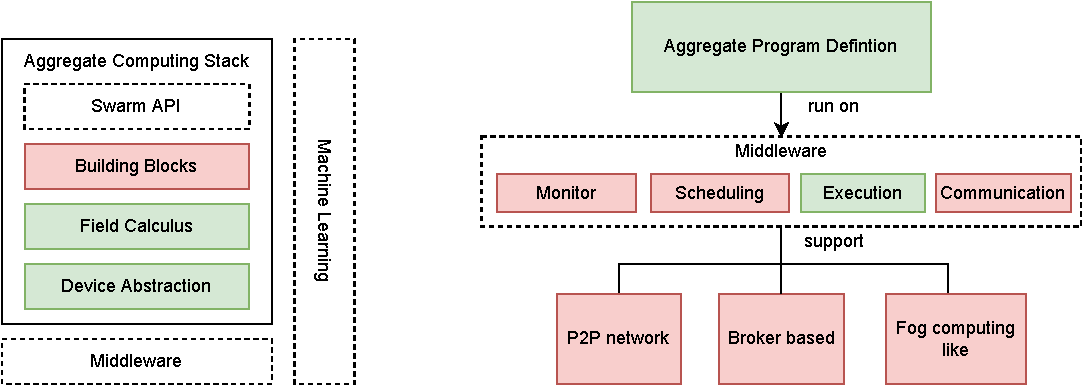
\includegraphics[width=0.9\textwidth]{img/to-do-for-thesis.pdf}
	\caption{Current status of \ac{ac} toolkit in literature. Dotted blocks mean a lack of that concept. Green blocks are the ones that can be considered stable and reusable in \acp{cpsw} engineering. Red blocks are the ones that currently exist but need to be expanded in order to support \acp{cpsw}.}
	\label{fig:current-state}
\end{figure}
\subsection{Preliminary contributions}
In my first year of PhD, my activities have been centred on
the integration of \ac{ac} with ML capability to create even more
intelligent collective behaviour. 
%
My works climaxes with ~\cite{research} where I explain different suitable approaches to
enhance \ac{ac} with ML. Finally, in the last period, I made concrete
experiments with Reinforcement Learning -- in particular, Hysteretic Q-Learning \cite{hysteretic-q} -- improving the current \ac{ac} solutions.

Concerning middleware aspects, my research activities aim at closing the gap between
its abstract space and its application in concrete systems. In this direction, I made mainly contributions to \scafi{}.
%
We have adopted \scafi{} mostly for practical reasons: concerning other aggregate programming languages such as Proto and Protelis, surveyed in \cite{viroli2019jlamp-si-coord},
\scafi{} is a \emph{strongly typed}, \emph{internal} DSL; therefore, it enables straightforward reuse of powerful features from the Scala host language (including its type system, type inference, programming abstractions, libraries).
%
Additionally, \scafi{} also represents an agile framework for testing experimental language features (cf. \emph{aggregate processes}~\cite{DBLP:journals/eaai/CasadeiVAPD21}.
%
Hence, among the existing languages for \ac{ac}, I believe that \scafi{} is the one better fitting for the rich scenarios of \acp{cpsw}.

The contributions done are described in two articles concerning ScaFi-Web -- a web-based tool that could support monitoring aspects and \scafi Loci -- a type-safe deployment methodology leveraging multitier programming.
\paragraph{ScaFi-Web -- A tool for a distributed monitoring} \label{scafi-web}
\scafiweb{}\footnote{\url{https://scafi.github.io/web}}~\cite{DBLP:conf/coordination/AguzziCMPV21}
 is an online playground for learning \ac{ac}, experimenting with it, and monitoring executions in a browser.
% a  web-based platform supporting \scafi{} in-browser that
It currently features:
\begin{itemize}
 \item an interactive editor for writing \scafi{} programs;
 \item a guided tour of the most prominent features, kickstarting development;
 \item an in-browser simulated network of devices hosting the execution;
 \item visualisation, inspection, and interaction tools integrated with the simulated environment.
\end{itemize}
%
Furthermore, it also provides a stepping stone towards a monitoring and control system for \ac{ac} deployments.
Indeed, in the context of field-based coordination, automated runtime verification approaches have been recently investigated~\cite{DBLP:journals/jss/AudritoCDSV21}, whereby spatial or temporal logics are mapped to field calculus programs to encode the behaviour of decentralised monitoring.
%
The \scafiweb{}'s frontend has been designed to be adaptable to different backends; indeed, the UI is completely separated from the underlying aggregate execution system. 

\paragraph{ScaFi Loci -- Towards a type-safe deployment of Pulverised Architecture}
\ac{ac} defines a conceptual model by which it is possible to define collective computation. Practically, each node needs to have a notion of the neighbourhood (i.e., which nodes are near to me). \textit{How} this neighbourhood has been built, is transparent for the computational model. Therefore it is possible to deploy the same application in different IT networks.
%
Pulverised architectures (i.e., pulverisation~\cite{DBLP:journals/fi/CasadeiPPVW20}) go in this direction, identifying the main \textit{deployable} units that can be moved in different concrete nodes, the core idea is that the functional behaviour of a distributed application is fundamentally orthogonal to the actual deployment of the services that compose it.
%
However, pulverisation does not specify how a pulverised architecture should
be described and verified so that it can be correctly operated at runtime.
Therefore, in \scafi{} Loci~\cite{DBLP:conf/acsos/AguzziCPSV21} I define an architecture for multitiered deployment strategies in pulverised systems, along with an implementation using ScaFi and ScalaLoci.
%
The latter enables a \textit{typesafe} multitier programming approach -- by which distributed architecture is defined
in a single compilation unit with a single language.
%
This work could be seen as a piece of flexible middleware that I intend to build, only focused on the deployment aspects.

\section{Future works}\label{future}
This section concludes the thesis proposal defining the next step of my PhD. In particular, I want to concretise the Reinforcement Learning and \ac{ac} integration (\Cref{rl-future}). Furthermore, I want to define a reusable API applied in \acp{cpsw} (\Cref{swarm-api}), and the first proof of concept of a flexible middleware by combing the first works done in my PhD (\Cref{middleware}). 
\subsection{Swarm API}\label{swarm-api}
The thesis will extend the current \ac{ac} stack with high-level API about swarms behaviours (Swarm API) like flocking, foraging, blinking, and spreading of information. The swarm API will not only mimic some nature-inspired behaviours, but it will give a general interface to solve common collective problems. The API should be reused in other contexts, such as collective adaptive systems (CAS), swarm robotics, or multi-agent systems.
To perform this abstraction layer definition I intend to:
\begin{itemize}
	\item perform a literature review of API/DSL for swarm robotics;
	\item identify common patterns;
	\item encode them in \ac{ac} framework and evaluate the performance through simulations.
\end{itemize}
\subsection{Reinforcement Learning applied to Building Blocks}\label{rl-future}
\ac{ac} bases its logic in \textit{compositionality} inspired by functional programming. The idea is that complex behaviours can be defined through the composition of \emph{building blocks}. Furthermore, based on these programming bricks, relevant collective properties are proven, such as self-stabilisation~\cite{DBLP:journals/corr/abs-1711-08297} and eventual consistency~\cite{DBLP:conf/saso/BealVPD16}. 
%
Currently, the problem with those building blocks is that they do not work well in any network topology. In literature, indeed, when we are dealing with high node dynamics, the overall computation field becomes quite noised and unstable -- leading to not reaching our intended result.
%
Traditionally, these problems are tackled with heuristics/algorithms that target a particular issue (stability of results, convergence speed up, \dots{}). However, this leads to complex parameters fine-tuning in each new environment.
%
Our hypothesis, described in~\cite{research}, consists of applying \ac{ml} algorithms -- and in particular Reinforcement Learning --
to speed up the self-stabilisation process of building blocks.

Applying \ac{rl} at this level is challenging due to non-fixed input (the neighbourhood is variable), multi-agent credit assignment problem (understanding the impact of one action giving a global utility), partial observability, very large state-action space, and distributed control.

These problems are partially tackled in different \ac{marl} algorithms, but a one-fit-for-all solution currently does not exist. Therefore, in the next two years I want to:
\begin{itemize}
	\item publish our first results using Hysteretic Q-Learning -- this will be a baseline;
	\item use Deep Learning techniques to handle large-action space;
	\item move our solutions from \emph{offline} to \emph{online} learning. 
\end{itemize}
In our early works, I focused on applying offline-\ac{rl} with a CTDE methodology.
Although, another thriving area is to use \emph{online} (continual) learning, so aggregate programs regularly adjust themselves to improve a global utility. Even if some approaches exist~\cite{DBLP:conf/icml/OmidshafieiPAHV17}, currently it is very challenging to apply online learning on such a large scale. Therefore probably it will be out-of-the-scope for this thesis, but it will be future work for continuing the integration \ac{ac} and \ac{rl} integration. 
\subsection{\emph{Intellingent} and \emph{Flexible} Middleware}\label{middleware}
\ac{ac} gives a theoretical framework by which it is possible to express composable collective behaviours. It abstracts over various aspects such as round frequency, neighbourhood discovery, and message delivery.
%%
One of the goals of this thesis is to concretise a software artefact -- middleware -- able to \emph{flexibly} and \emph{smartly} manage the aforementioned aspects.
%
The core idea is to leave unspoilt the high-level program specification (expressed which aggregate programming) and endow the burden to the middleware of accomplishing some QoS by fine-tuning the architectural aspects. 
%
In this way, I promote a design process in which:
\begin{itemize}
	\item the designers express the collective behaviour once and thinking about computational fields;
	\item the middleware configures the underlying aspect to support the same computation in different scenarios.
\end{itemize}
%
In the \ac{ac} literature, several works follow this idea. 
%
For instance, the \emph{distributed schedulers}~\cite{DBLP:journals/corr/abs-2012-13806} aim at efficiently managing device scheduling using the same abstraction as \ac{ac}.
Instead, the pulverisation~\cite{DBLP:journals/fi/CasadeiPPVW20} approach aims at adapting aggregate computation to any kind of deployment.
%
The middleware will contain these ideas, seamlessly integrated with \ac{rl} techniques as an inherent technique for achieving  QoS constraints.
%
Taking the example of the scheduler, in our vision, \ac{rl} could be used to autonomously tune the overall system frequency through a global utility optimisation, reducing the complexity in configuring the scheduling policy.
%
Definitely, \emph{learning} should be a key concept to create flexible middleware necessary to \acp{cpsw}, and hence it will be a part of my thesis work. 
\nocite{collectiveautonomy}
\section{Published papers}
\printbibliography[heading=none, check=mine]
\section{References}
\printbibliography[heading=none, check=other]

\end{document}